\documentclass[10pt,a4paper]{article}
\usepackage[utf8]{inputenc}
\usepackage[T1]{fontenc}

%\usepackage[showframe]{geometry}

\usepackage[
backend=bibtex,
sorting=ynt
]{biblatex}
\addbibresource{refs.bib}

\defbibheading{secbib}[\bibname]{%
	\section*{#1}%
	\markboth{#1}{#1}}

\usepackage{graphicx}
\usepackage{subfig}
\usepackage{todonotes}
\usepackage{amsfonts}
\usepackage{amsmath}
\usepackage{amssymb}
\usepackage{amsthm}
\usepackage{hyperref}
\usepackage[capitalise, noabbrev]{cleveref}
\usepackage{float}
\usepackage{mathbbol}
%\usepackage{tikz-cd}
\usepackage{tikz}
\usepackage{enumitem}
\usepackage{xcolor}
\usepackage{tcolorbox}
\tcbuselibrary{breakable}

\usepackage{newpxtext,newpxmath} % Should be the last package import

\theoremstyle{definition}
\newtheorem{thm}{Theorem}[section]
\newtheorem{defn}[thm]{Definition}
\newtheorem{lem}{Lemma}[thm]
\newtheorem{cor}{Corollary}[thm]
\newtheorem{prop}{Proposition}[thm]
\newtheorem{rem}{Remark}[thm]
\newtheorem{ill}{Illustration}[thm]
\newtheorem{ex}{Example}[thm]

\newcommand{\conv}[1]{\ensuremath{\operatorname{conv}(#1)}}
\newcommand{\posreals}{\ensuremath{\mathbb{R}_{>0}}}
\newcommand{\R}{\mathbb{R}}
\newcommand{\pers}{\mathcal{D}}

\newenvironment{idea}{%
	\begin{tcolorbox}[colback=green, breakable, sharp corners]
		\textbf{Idea: }
		\medskip
		\begin{quote}
			\centering
}{\end{quote}\medskip\end{tcolorbox}}


\setlength\parindent{0pt}

\linespread{1.5}

\title{Summary: Outlier Robustness}
\begin{document}
\maketitle

%Given a finite point cloud $X\subset\R^d$, we are interested in capturing how the removal (or addition) of an outlier point affects the persistent homology module. Suppose $x_0\in X$ and write $X_0 = X\setminus\{x_0\}$. The classical stability results in Topological Data Analysis (TDA) provide stability with respect to the Hausdorff distance. That is, the interleaving distance between the Čech homology groups of $X$ and $Y$ are bounded by the distance $d_H(X,Y)$. This guarantees stability with respect to small permutation of the point cloud. But adding a single point can move us far away from the initial point cloud, and consequently, classical stability does not help much with outlier robustness. Several alternative constructions have been proposed to deal with this problem. These includes \todo{add references} ...

\begin{abstract}
	This note is an attempt to summarise some of the articles and constructions we have been looking at in previous meetings. I will also try to summarise what kind of outlier robustness (leave-one-out stability) these methods are guaranteed to have.
\end{abstract}

\textbf{Some fixed notation:} Given a (finite) point cloud $X$ with $|X|=n$, let $\mu_X$ denote the empirical probability measure with support on $X$. That is, $\mu_X = \frac{1}{n}\sum_{x\in X}\delta_x$ where $\delta_x$ denotes the Dirac measure centred at $x$. Similarly, let $\mu_{X_0}$ denote the empirical measure on $X_0 = X\setminus\{x_0\}$ for some arbitrary $x_0\in X$. 

%We consider two distance functions on probability measures. Namely, the $p$-Wasserstein distance $W_p$ and the Prohorov distance $d_{Pr}$.

\section{Hausdorff distance and outliers}
Stability in topological data analysis often refers to the robustness of topological features with respect to small perturbations in the data. We will refer to this type of stability as \textit{classical stability}. However, classical stability is not sufficient to provide robustness against outliers. Given two subsets $A$ and $B$ of a metric space $(Y,d)$, the \textit{Hausdorff distance between $A$ and $B$}, denoted $d_H(A,B)$ is defined as
$$
d_H(A,B) = \inf\{\epsilon\geq0\mid A\subseteq B^\epsilon\text{ and }B\subseteq A^\epsilon\}
$$
where $X^\epsilon = \{y\in Y\mid d(y,x)\leq\epsilon\text{ for some }x\in X\}$ is the $\epsilon$-thickening of $X$ with respect to $d$. \Cref{fig:thickening_of_torus} illustrates the thickening of a point cloud sampled uniformly from the $2$-torus embedded in $\R^3$.

\begin{figure}[H]
	\centering
	\begin{tabular}{cccccc}
		\subfloat{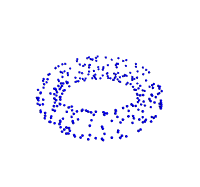
\includegraphics[width = 0.650in]{figs/thick_torus_1.png}} &
		\subfloat{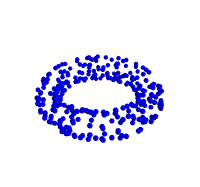
\includegraphics[width = 0.650in]{figs/thick_torus_2.png}} &
		\subfloat{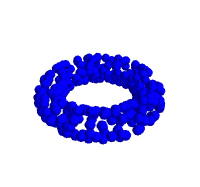
\includegraphics[width = 0.650in]{figs/thick_torus_3.png}} &
		\subfloat{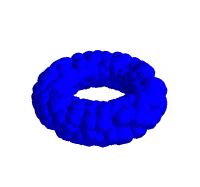
\includegraphics[width = 0.650in]{figs/thick_torus_4.png}} &
		\subfloat{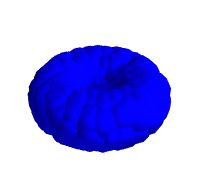
\includegraphics[width = 0.650in]{figs/thick_torus_5.png}} &
		\subfloat{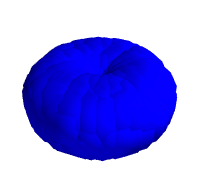
\includegraphics[width = 0.650in]{figs/thick_torus_6.png}}
	\end{tabular}
	\caption{The $\epsilon$-thickening of a point cloud sampled from a $2$-dimensional torus. Here $\epsilon$ increases as we go from left to right.}\label{fig:thickening_of_torus}
\end{figure}

For a point $y\in Y$ and a subset $X\subseteq Y$ we write $d(y,X)=\inf_{x\in X} d(y,x)$ and $d(-,X)$ for the function $y\mapsto d(y,X)$. The Hausdorff distance can then be written in the following two forms equivalent to the above definition:
$$
d_H(A,B) = \max\left\{\sup_{a\in A}d(a,B), \sup_{b\in B}d(b,A)\right\} = \Vert d(-,A) - d(-, B)\Vert_\infty.
$$

Given a function $f\colon Y\to\R$, we denote by $\operatorname{Dgm}(f)$ the persistence diagram of the sublevel sets of $f$. The persistence diagram $\operatorname{Dgm}(f)$ encodes the birth and death times of generators of $H_k(f^{-1}(-\infty, t])$ for all values of $t\in\R$ and integers $k\geq 0$. In other words, $\operatorname{Dgm}(f)$ records the topological features of the sublevels sets of $f$ that persists when we vary $t$. There is a correspondence between persistence diagrams and what we call barcodes. There is a subtle difference in that barcodes contains information about whether or not the persistence intervals includes its endpoints. This difference can be important but in our case where we consider the homology of sublevel sets it does not matter so we view persistence diagrams and barcodes as representations of the same thing. Moreover, by the decomposition theorem in \autocite{Crawley2012}, every persistence module (of finite type) is completely characterized (up to isomorphism) by its corresponding barcode. The following result makes stability with respect to perturbation of the input data (or functions) precise:
\begin{prop}[Classical stability. See \autocite{cohen2005stability} and \autocite{Chazal2012}]
	Let $f,g\colon Y\to\R$ be continuous and tame\footnote{A function $f\colon Y\to\R$ is said to be \textit{tame} if the homology groups of its sublevel sets are finite in all degrees and $f$ has a finite number of homological critical values. See \autocite{cohen2005stability} for precise definitions.} functions with $X$ triangulable. Then $d_I(\operatorname{Dgm}(f), \operatorname{Dgm}(g))\leq\Vert f-g\Vert_\infty$.
\end{prop}

Now, for a point cloud $X\subseteq Y$, consider the distance function $f=d(-,X)$ and observe that for any $t\geq 0$, we have
$$
X^t := f^{-1}(-\infty, t] = \left\{y\in Y\mid\exists x\in X\text{ s.t. }d(x,y)\leq t\right\} = \bigcup_{x\in X}B(x,t).
$$
In other words, the $t$-sublevel set of $f$ is the $t$-thickening of $X$. Since $X^t\subseteq X^s$ for $t\leq s$, we obtain a filtered topological space $\left\{X^t\right\}_{t\geq 0}$ called the \textit{Čech filtration} of $X$. Given a cover $\mathcal{U}=\{U_i\}_{i\in I}$ of a topological space $Z$, we define the \textit{nerve of $\mathcal{U}$}, denoted $\mathcal{N}(\mathcal{U})$, to be the simplicial complex with vertex set $I$ defined by
$$
\sigma = \{i_0, i_1, \ldots, i_k\}\in\mathcal{N}(\mathcal{U})\iff \bigcap_{i\in\sigma}\neq\emptyset
$$
If for all finite non-empty $J\subseteq I$, the intersection $\bigcap_{i\in J} U_i$ is non-empty, the \textit{nerve theorem} states that $\mathcal{N}(\mathcal{U})$ is homotopy equivalent to $Z=\bigcup_{i\in I}U_i$. The family $\left\{B(x,t)\right\}_{x\in X}$ defines a cover of $X^t$ for every $t\geq 0$. Taking the nerve of the cover $\left\{B(x,t)\right\}_{x\in X}$, we obtain a simplicial complex $\operatorname{\text{\v{C}ech}}_t(X)$ with vertex set $X$. Applying this construction for different values of $t$, we get a filtered simplicial complex $\operatorname{\text{\v{C}ech}}(X) =\left\{ \operatorname{\text{\v{C}ech}}_t(X)\right\}_{t\geq 0}$ called the \textit{Čech complex of $X$}. By the nerve theorem, we have that the Čech filtration and the Čech complex of $X$ are homotopy equivalent, and hence they have isomorphic persistent homology modules. If we let $\operatorname{Dgm}^{\text{Č}}(X)$ denote the persistence diagram corresponding to the persistent homology of $\operatorname{\text{\v{C}ech}}(X)$, the classical stability theorem can now be written as 
$$
d_I(\operatorname{Dgm}^{\text{Č}}(X), \operatorname{Dgm}^{\text{Č}}(Y))\leq\Vert d(-,X) - d(-, Y)\Vert_\infty = d_H(X,Y).
$$
We now consider an simple example to demonstrate the above construction's sensitivity to outliers. 
\begin{figure}[H]
	\centering
	\begin{tabular}{ccc}
		\subfloat{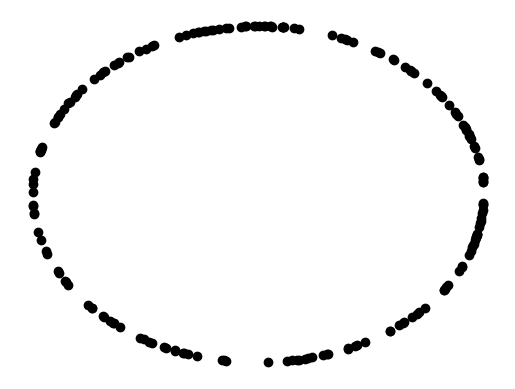
\includegraphics[width = 1.4in, height = 1.4in]{figs/0_point_cloud.png}}&
		\subfloat{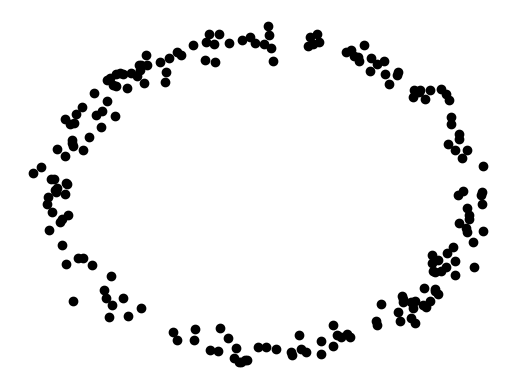
\includegraphics[width = 1.4in, height = 1.4in]{figs/1_point_cloud.png}}&
		\subfloat{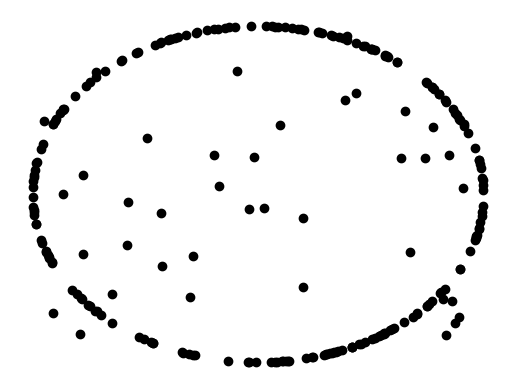
\includegraphics[width = 1.4in, height = 1.4in]{figs/3_point_cloud.png}}\\
		$X_0$ & $X_1$ & $X_2$
	\end{tabular}
	\caption{Three point clouds resembling a circle in the plane. The point cloud $X_0$ consists of points sampled uniformly from $S^1$, whereas $X_1$ is a slightly perturbed version of $X_0$, and $X_2$ is $X_0$ with a small number of outliers added.}\label{fig:clean_perturbed_noisy_circles}
\end{figure}
The Hausdorff distance between $X_0$ and $X_1$ is small, whereas $d_H(X_0, X_2)$ is large in comparison. \Cref{fig:clean_perturbed_noisy_circles_pers_diagrams} shows the corresponding persistence diagrams. As expected by the classical stability theorem, the diagrams corresponding to $X_0$ and $X_1$ are similar and both captures the homology of the underlying circle. However, the diagram of $X_2$ exhibits a lot of noise and it is not possible to infer the topology of a circle from the diagram.
\begin{figure}[H]
	\centering
	\begin{tabular}{ccc}
		\subfloat{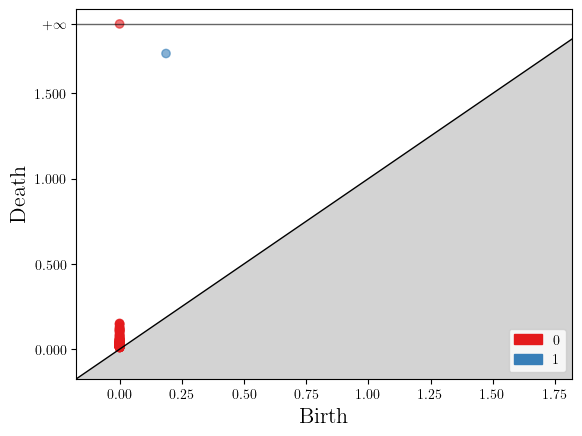
\includegraphics[width = 1.4in, height = 1.4in]{figs/0_diagram.png}}&
		\subfloat{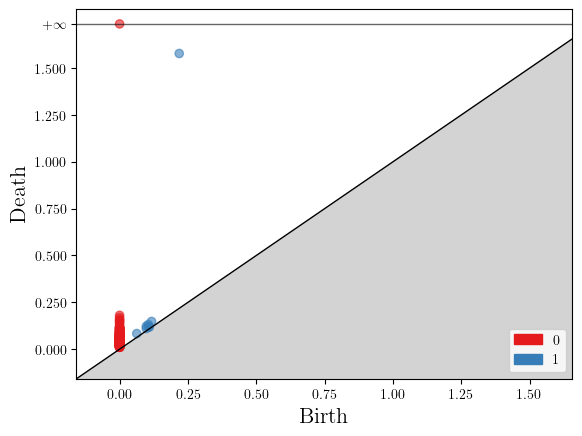
\includegraphics[width = 1.4in, height = 1.4in]{figs/1_diagram.png}}&
		\subfloat{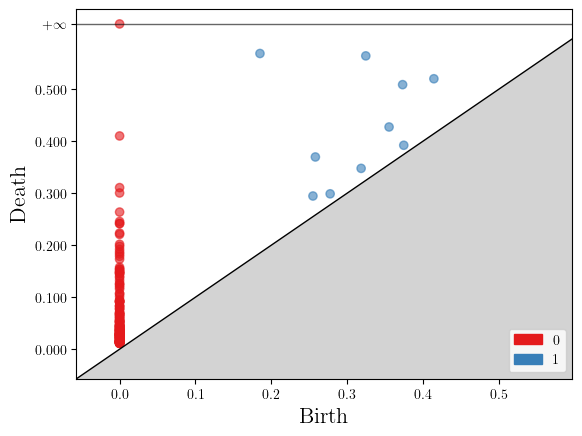
\includegraphics[width = 1.4in, height = 1.4in]{figs/3_diagram.png}}\\
		$\operatorname{Dgm}^{\text{Č}}(X_0)$ & $\operatorname{Dgm}^{\text{Č}}(X_1)$ & $\operatorname{Dgm}^{\text{Č}}(X_2)$
	\end{tabular}
	\caption{Three point clouds resembling a circle in the plane. The point cloud $X_0$ consists of points sampled uniformly from $S^1$, whereas $X_1$ is a slightly perturbed version of $X_0$, and $X_2$ is $X_0$ with a small number of outliers added.}\label{fig:clean_perturbed_noisy_circles_pers_diagrams}
\end{figure}

\subsubsection{Previous work}
\todo[inline]{What have been done to make PH robust against outliers? Specifically, density based methods. Constructions that takes the density in local neighbourhoods of $X$ into consideration. Potential problems: (1) Computability in practice. (2) Additional parameters for which there is no obvious way to pick the best value.}


\section{Uniform stability}
Let $Y$ be a metric space, and consider a function $V$ taking a finite subset $X\subseteq Y$ to a persistence module $V_X$. We introduce the notion of uniform stability for such functions with inspiration from learning theory (cf. \cite{bousquet2002stability}). If $X\subseteq Y$ is a point cloud and $x_0\in X$, we fix the notation $X_0 = X\setminus\{x_0\}$. The intuition behind uniform stability is that, given enough samples, the difference between $V_X$ and $V_{X_0}$ should be very small.

\begin{defn}\label{def_uniform_stability}
	We say that $V$ is \textit{uniformly stable with respect to $d$} if for every finite subset $X\subseteq Y$ with $|X|=n$, there exists a positive real number $\beta(n)\in\mathcal{O}(n^{-1})$ such that
	\begin{equation}\label{eq_uniform_stability}
		 d\left(V_X,\,V_{X_0}\right) \leqslant \beta(n)\quad\text{holds for all }x_0\in X.
	\end{equation}
\end{defn}

%For $1$-parameter persistent homology, we can take $d$ to be the usual interleaving distance $d_I$ between persistence modules. By the isometry theorem of \autocite{Bauer2015}, this distance agrees with the bottleneck distance between barcodes/persistence diagrams. The interleaving distance extends to $2$-parameter persistence modules which allows us to talk about uniform stability in the $2$-parameter setting as well. In practice, one does not necessarily prove stability directly on the algebraic level of persistence modules, but rather on the level of (bi-)filtrations of topological spaces or simplicial complexes.

\begin{rem}
The following three observations follows readily from the triangle inequality:
\begin{enumerate}
	\item \textbf{Removal of multiple points:} Let $X_k=X\setminus\{x_0, x_1,\ldots x_k\}$ for some  $x_0,x_1,\ldots,x_k\in X$. If $V$ is uniformly stable, then $d\left(V_X, V_{X_k}\right)$ is also bounded by some $\beta(n)\in\mathcal{O}(n^{-1})$.
	\item \textbf{Replacing a point:} If $X'=(X\setminus\{x_0\})\cup\{x'\}$ for some $x'\in Y$, then $d\left(V_X, V_{X'}\right)$ is also bounded by some $\beta(n)\in\mathcal{O}(n^{-1})$.
	\item \textbf{Interleavings and stability (?) :} If $V$ and $W$ are $\epsilon$-interleaved and $V$ is uniformly stable with respect to the interleaving distance $d_I$, then $d_I\left(W_{X}, W_{X_0}\right)\leq2\epsilon+\beta(n)$.
\end{enumerate}
\end{rem}
\begin{proof}\,
	\begin{enumerate}
		\item By the triangle inequality and uniform stability of $V$, we have that $$d(V_X, V_{X_k})\leq d(V_{X}, V_{X_{k-1}})+d(V_{X_{k-1}}, V_{X_{k}})\leq d(V_{X}, V_{X_{k-1}})+\beta(n),$$ so the claim follows by induction.
		\item Since $X_0=X'\setminus\{x'\}$, it follows that
		\begin{align*}
			d(V_X,V_{X'})&\leq d(V_X,V_{X_0})+d(V_{X'\setminus\{x'\}},V_{X'})\leq2\beta(n).%\max\left\{\beta(n),\,\beta'(n)\right\}.
		\end{align*}
		\item From the assumptions we have $d_I(V_X, V_{X_0}) \leq \beta(n)\in\mathcal{O}(n^{-1})$ and $d_I(V_Z, W_Z)\leq\epsilon$ for all $Z$. Using the triangle inequality, we have
		\begin{align*}
			d_I(W_X, W_{X_0}) &\leq d_I(W_X, V_X) + d_I(V_X, W_{X_0})\\
			&\leq \epsilon + d_I(V_X, V_{X_0})) + d_I(V_{X_0}, W_{X_0})\leq 2\epsilon + \beta(n).
		\end{align*}
	\end{enumerate}
\end{proof}

\subsection{The multicover bifiltration and the Prohorov distance}
The \textit{offset filtration} $O(X)$ of a point cloud $X$ is a filtered topological space given in filtration degree $r>0$ as the union of all balls of radius $r$ centred at the points in $X$. Taking the nerve of this collection of balls of radius $r$, we get the usual Čech filtration. The multicover bifiltration $\mathcal{M}(X)$ is a $2$-parameter extension of the offset filtration which is sensitive to density. Given a metric measure space $(Y,\eta_Y)$, the \textit{measure bifiltration $\mathcal{B}(Y)$} is given in filtration degree $(k,r)$ by $$\mathcal{B}(Y)_{(k,r)}=\{y\in Y\mid\eta_Y(B(y,r))\geq k\}.$$
For a point cloud $X\subseteq\R^d$, the \textit{unormalized multicover bifiltration $\mathcal{M}^u(X)$} of $X$ is then defined as $\mathcal{M}^u(X)=\mathcal{B}(\hat{\nu}_X)$ where $\hat{\nu}_X$ is the counting measure on $X$ defined as $\hat{\nu}_X(A)=|A\cap X|$. In other words, $\mathcal{M}^u(X)_{(k,r)}$ consists of all $y\in \R^d$ such that the ball centred at $y$ of radius $r$ contains at least $k$ distinct points $x$ from $X$. The \textit{(normalized) multicover filtration $\mathcal{M}(X)$} is defined similarly by replacing $\hat{\nu}_X$ with the empirical probability measure $\nu_X(A)=|A\cap X|/|X|$. This normalizes the first parameter $k$ by the number of points in $X$.


The \textit{Prohorov distance} $d_{Pr}$ between two (probability) measures $\mu$ and $\eta$ on a metric space $(Y,d_Y)$ is given by
$$
d_{Pr}(\mu, \eta) = \sup_A\inf\{\delta\geq0\mid\mu(A)\leq\eta(A^\delta)+\delta\text{ and } \eta(A)\leq\mu(A)+\delta\}
$$
where $A$ ranges over all closed sets in $Y$. The notation $A^\delta$ means the $\delta$-thickening of $A$ in $Y$ with respect to the metric $d_Y$. It follows from remark 2.16 in \cite{Blumberg2020} that the Prohorov distance between the two empirical probability measures $\mu_X$ and $\mu_{X_0}$ is bounded above by $\frac{1}{n-1}$. The following special case of a theorem of \cite{Blumberg2020} then implies uniform stability for the multicover bifiltration with respect to the interleaving distance for 2-parameter persistence modules.

\begin{thm}[Theorem~1.6~\cite{Blumberg2020}]
For $X$ and $X'$ non-empty, finite subsets of $\mathbb{R}^d$,
$$
d_I(\mathcal{M}(X), \mathcal{M}(X'))\leq d_{Pr}(\mu_X, \mu_{X'}).
$$
\end{thm}

\todo[inline]{\textbf{Todo:} Look at the subdivision and degree bifiltrations and understand how these are related to the multicover bifiltration. The paper \autocite{Rolle22} an example exploring stability of degree-Rips on an annulus with outliers.}

\begin{ex}
	The Hausdorff distance between two point clouds is \textit{not} bounded below by the Prohorov distance between their associated empirical measures. In other words, stability with respect to the Prohorov distance does not in general imply stability with respect to the Hausdorff distance. To see this, consider the following simple example: Given any $\epsilon\in(0,\frac{1}{2})$, let $X=\{x,y\}$ such that $d(x,y)>1$ and let $X'$ be the union of $X$ and a collection of points $\{x_1, x_2,\ldots,x_N\}$ with all $x_i\in B(y,\epsilon)$. Then, clearly the Hausdorff distance $d_H(X,X')\leq\epsilon$. Suppose that $\delta = d_{Pr}(\mu_X, \mu_{X'})\leq\epsilon$. Then for $A=\{x\}$ we have $A^\delta=A$ so by the definition of the Prohorov distance the inequality $\mu_X(A)\leq\mu_{X'}(A^\delta)+\delta$ holds. This implies that $\frac{N+1}{N+2}\leq\delta\leq\epsilon$ which is absurd since $\epsilon<\frac{1}{2}$. Hence, we must have that $d_{Pr}(\mu_X, \mu_{X'})>d_H(X,X')$.
\end{ex}

\subsection{The Wasserstein distance}
The Wasserstein distance, also known as the Earth Mover's Distance, is a distance measure between probability measures. It can be used to compare the similarity between two distributions, with smaller values indicating greater similarity. Some methods proposed in TDA for dealing with noise and outliers gives guarantees in terms of the Wasserstein distance. For two probability measures $\mu$ and $\eta$ on $Y=\R^d$, we define the \textit{$p$-Wasserstein distance} between $\mu$ and $\nu$ to be
$$
W_p(\mu, \eta) = \inf_{\nu}\left(\int_{Y\times Y}\Vert x-y\Vert^p d\nu\right)^{\frac{1}{p}}.
$$
Here, $\nu$ ranges over all couplings of $\mu$ and $\eta$. A coupling is a joint probability distribution on $Y\times Y$ with marginals equal to $\mu$ and $\eta$, respectively. Such couplings are also often referred to as transport plans, and one minimizing the above expression is called an optimal transport plan. For two measures $\mu$ and $\eta$ with finite support, a transport plan can be represented as a matrix $A=(a_{ij})$ where $a_{ij}$ is the mass moved from $x_j$ to $x_i$. In this case, the $p$-Wasserstein distance between $\mu$ and $\eta$ is given as
$$
W_p(\mu, \eta) = \inf_A \left(\sum_{i,j}\Vert x_j - y_i\Vert^p\cdot a_{ij}\right)^{\frac{1}{p}}.
$$

For example, let $\mu_X$ and $\mu_{X_0}$ be the empirical measures with support $X$ and $X_0$, respectively. One way to think about transport plans between $\mu_X$ and $\mu_{X_0}$ is as follows: If we add a point $x_0$ to go from $X_0$ to $X$, each of the other $n-1$ points have to give away some mass so that all points, including $x_0$, ends up with a mass of $\frac{1}{n}$. One possible transport plan is given by the $(n-1)\times n$-matrix
$$
	\begin{bmatrix} 
	\frac{1}{n(n-1)} & \frac{1}{n} & 0 & 0 & \dots  & 0 & 0\\
	\frac{1}{n(n-1)} & 0 & \frac{1}{n} & 0 & \dots  & 0 & 0\\
	\vdots & \vdots & \vdots & \vdots & \ddots & \vdots & \vdots \\
	\frac{1}{n(n-1)} & 0 & 0 & 0 & \hdots & \frac{1}{n}  & 0 \\
	\frac{1}{n(n-1)} & 0 & 0 & 0 & \hdots & 0 & \frac{1}{n}  \\
	\end{bmatrix}
$$
Since the Wasserstein distance is the infimum over all such transport plans, we have the following upper bound
\begin{align*}
W_p(\mu_X, \mu_{X_0})&\leq \left(\frac{1}{n(n-1)}\sum_{x\in X_0}\Vert x_0-x\Vert^p\right)^{\frac{1}{p}} \\&\leq\left(\frac{n-1}{n(n-1)}\operatorname{diam}(X)^p\right)^{\frac{1}{p}} = n^{-\frac{1}{p}} \operatorname{diam}(X).
\end{align*}

\begin{idea}
	Can we find a tighter bound for $d_W(\mu_X, \mu_{X_0})$?
\end{idea}

Assuming that the diameter of $X$ does not depend on $|X|$, the above inequality implies that the $1$-Wasserstein distance between $\mu_X$ and $\mu_{X_0}$ is $\mathcal{O}(n^{-1})$.

\subsubsection{The distance to a measure (\autocite{Buchet2013})}
For a probability measure $\mu$ on a metric space $Y$ and a mass parameter $m\in(0,1]$, define the function $\delta_{m,\mu}\colon\R^d\to\R_{>0}$ by sending a point $y$ in $\R^d$ to the real number $\inf\{r>0\mid\mu(\bar{B}(y,r))>m\}$. Intuitively, $\delta_{m,\mu}$ describes how large a disk around $y$ we have to consider to capture at least $m$ mass as defined by $\mu$. Using $\delta$, we define \textit{the distance $d_{\mu,m}$ to measure $\mu$} as
\begin{align*}
	d_{\mu,m}\colon\R^d&\to\R_{>0}\\
	y&\mapsto\sqrt{\frac{1}{m}\int_0^m\delta_{mu,l}(x)^2dl}.
\end{align*}

Let $\operatorname{Dgm}(d_{\mu,m})$ denote the persistence diagram corresponding to the sublevel set homology of $d_{\mu,m}$. In \autocite{Buchet2013}, the following Wasserstein stability result is established for the distance to a measure function:
\begin{thm}[Theorem~3.1~\autocite{Buchet2013}]
	For two probability measures $\mu$ and $\nu$ and a triangulable metric space $Y$ and a mass parameter $m$, we have that
	$$
	d_B(\operatorname{Dgm}(d_{\mu,m}), \operatorname{Dgm}(d_{\nu,m})) \leq \frac{1}{\sqrt{m}}W_2(\mu, \nu).
	$$
\end{thm}

In particular, for the empirical measures $\mu_X$ and $\mu_{X_0}$ this implies
$$
d_B(\operatorname{Dgm}(d_{\mu_X,m}), \operatorname{Dgm}(d_{\mu_{X_0},m})) \leq \frac{1}{\sqrt{n}}\frac{1}{\sqrt{m}}\operatorname{diam}(X).
$$

\textbf{Approximation via a weighted Čech (or Rips) complex}
\todo[inline]{\textbf{Todo:} Write something about stability in case of the complex used to approximate DTM. See \autocite{Anai2018}. There are also some stability results wrt. the Wasserstein distance in \autocite{Anai2018}.}
Computing the sublevel set homology of $d_{\mu, m}$ in practice is difficult. In \autocite{Hoefgeest2022} the authors propose a way to approximate the sublevel set homology by using weighted complexes.

\subsubsection{Christoffel polynomials \autocite{Hoefgeest2022}}
In the paper \autocite{Hoefgeest2022}, the authors investigate use of Christoffel polynomials to achieve robustness to outliers in the input data. Given a point cloud $X$, one is interested in the sublevel set persistent homology module $\mathbb{CD}(X,k)$ of the logarithm\footnote{The sublevel sets of $\log P_k^{\mu_X}$ rather than $P_k^{\mu_X}$ are considered. The rationale given in the original paper is that this allows for stronger and more elegant stability results, and also that the logarithmic scaling produces persistence diagrams that better fit the underlying topology. See page 8 of \autocite{Hoefgeest2022}.} of the Christoffel polynomial $P_k^{\mu_X}$ of degree $k$ induced by the empirical measure on $X$. Stability results are given with respect to the $1$-Wasserstein measure. %We note that the point cloud is assumed to be contained in the cube $[-1,1]^d\subset\R^d$ (scaling the data first if necessary).
The following stability result is established in \autocite{Hoefgeest2022}:
% variable names:
% paper	<-> here
% ---------------
% d 	<-> k
% n 	<-> d

\begin{prop}
	Let $X$ and $Y$ be point clouds in $[-1,1]^d$. Then,
	$$
	d_B\left(\operatorname{Dgm}(\mathbb{CD}(X,k)), \operatorname{Dgm}(\mathbb{CD}(Y,k))\right)\leq\log(C_X d_W(\mu_X, \mu_Y)+1)
	$$
	whenever $C_X\cdot d_W(\mu_X, \mu_Y)\leq 1$. Here $C_X = 2C_{d,k}\Vert P_k^{\mu_X}\Vert_\infty$ where $C_{d,k} = 4\binom{d+k}{k}k^2$.
\end{prop}

Consider $X$ and $X_0$ with their empirical measures $\mu_X$ and $\mu_{X_0}$, respectively. Since $\operatorname{diam}[-1,1]^d = 2\sqrt{d}$ we have the upper bound $\log\left(2n^{-1}\sqrt{d}C_X+1\right)$ for the bottleneck distance.


\subsubsection{Kernel density estimation}
Kernel density estimation is a non-parametric statistical technique for estimating the underlying probability density. It involves placing a kernel function, which is typically a smooth, continuous curve such as a normal distribution, at each data point and summing all of these kernel functions to estimate the true density function. The smoothness of the resulting curve is controlled by a parameter called the bandwidth. Sublevel set persistent homology can be applied to a kernel density estimator (KDE) to identify topological features in the data.

\begin{defn}
	Let $x$ be a point in $Y$. A \textit{kernel $g$ centred in $x$} is a function $g\colon Y\to\posreals$ with $g(y)=h\left(\Vert x-y\Vert\right)$ for some continuous function $h\colon[0,\infty)\to\posreals$. In addition, we require $h$ to be differentiable on $(0, \infty)$ with $h'(t)<0$. We call $h$ the \textit{height function} associated to $g$.
\end{defn}

Given a kernel $g$ centred in $0$, we denote by $g_x$ the shifted kernel given by $g_x(y)=g(x-y)$. If $X$ is a finite point cloud, we define the \textit{kernel density estimator (KDE) on $X$} (with kernel $g$) to be the function $f_X=\frac{1}{n}\sum_{x\in X}g_x\colon Y\to\posreals$. Showing that sublevel set homology of a kernel density estimator is uniformly stable is straight-forward.

\begin{prop}
	The function taking a point cloud $X$ to the sublevel set persistent homology of $f_X$ is uniformly stable.
\end{prop}
\begin{proof}
	Let $f_X$ and $f_{X_0}$ be the kernel density estimators with kernel $g$ on $X$ and $X_0$, respectively.
	\begin{align*}
		f_X - f_{X_0} &= \frac{1}{n}g_{x_0} -\frac{1}{n(n-1)}\sum_{x\in X_0}g_x
		= \frac{1}{n}\left(g_{x_0} - f_{X_0}\right). \\
	\end{align*}
	Consequently, we have that $\Vert f_X - f_{X_0}\Vert_\infty\in\mathcal{O}(n^{-1})$ and hence uniform stability follows from classical stability of persistence diagrams (cf. \autocite{cohen2005stability}).
\end{proof}

\textbf{A grid based approach to computing the sublevel set homology}

One practical challenge with a KDE based approach is to compute the persistence homology. For low dimensions such as $d=1$ and $2$, a piecewise linear approximation using a grid can be used. However, this approach depends on the grid resolution, and the number of vertices increases exponentially in the number of dimensions which makes it unfeasible for higher dimensional data. The following approximation scheme is used by \autocite{Hoefgeest2022} to compute the sublevel set homology of a Lipschitz continuous function $f\colon[-1,1]^d\to\R$:
\begin{enumerate}
	\item Fix a positive integer $m$ and construct the Freudenthal triangulation $\mathcal{K}_m$ of $[-1,1]^d$.
	\item This gives us a vertex set, with $(m+1)^d$ vertices, equal to the lattice points of $\frac{2}{m}\cdot\mathbb{Z}^n$.
	\item Evaluate $f$ on each vertex and compute the persistent homology module of the lower-star filtration on $\mathcal{K}_m$ induced by these function values. Denote the persistence diagram of this persistence module by $\operatorname{Dgm}(f\vert_{\mathcal{K}_m})$.
\end{enumerate}
The following proposition gives an upper bound on the error of this approximation in terms of the Lipschitz constant for $f$:
\begin{prop}[Proposition~22~\autocite{Hoefgeest2022}]
	Let $f\colon[-1,1]^d\to\R$ be Lipschitz continuous with Lipschitz constant $L_f$. Then
	$$
	d_B\left(\operatorname{Dgm}(f\vert_{\mathcal{K}_m}), \operatorname{Dgm}(f)\right)\leq \frac{2L_f\sqrt{d}}{m}
	$$
\end{prop}

\begin{idea}
	We know that all interesting topology of the sublevel sets of $f_X$ is contained in the convex hull of $X$. If we consider a triangulation of the convex hull (e.g., the Delaunay triangulation or some refinement of it), can we give guarantees for the approximation using the lower-star filtration on this triangulation? (See proof and discussion in Appendix B of \autocite{Hoefgeest2022}).
\end{idea}

\begin{idea}
	Can we first use a grid, and then apply some sparsification method (with approximation guarantees) to reduce the number of vertices?
\end{idea}

\printbibliography
\end{document}